\chapter{Methodology}
To accomplish the swing-up task, we utilize the Soft Actor-Critic, a classic model-free reinforcement learning algorithm. This trains a policy that can guide the system to the region of attraction (RoA) of a continuous-time linear quadratic regulator (LQR) controller. Once the system is within the RoA, we switch to the LQR controller to achieve full stabilization.

\section{Soft actor critic}
Within the landscape of reinforcement learning, the Soft Actor Critic (SAC) stands out as an algorithm specifically designed for environments with continuous action spaces. Such environments, exemplified by our double pendulum system where actuators can be adjusted to any value within the torque limit range, influenced our decision to adopt SAC.

Like many other deep reinforcement learning algorithms, SAC optimizes a policy by maximizing the expected cumulative reward the agent obtains over time. This optimization is primarily achieved through an actor-critic structure.

The actor determines the best actions by interpreting the current environmental conditions and adhering to the existing policy. Typically, the actor is visualized as a shallow neural network that approximates the mapping between the input state and the output probability distribution over actions. Furthermore, SAC incorporates a stochastic policy within its actor, which fosters exploration and aids the agent in refining its policies.

On the other hand, the critic evaluates the value of state-action pairs. It estimates the expected cumulative reward the agent can achieve by following a particular policy. More often than not, the critic is depicted as a neural network that processes state-action pairs as inputs to yield the estimated value.

A distinguishing feature of SAC, besides the actor-critic framework, is entropy regularization. SAC utilizes a stochastic policy. This means that instead of always settling on a single best action for each state, the agent considers a probability distribution over potential actions. The incorporation of entropy in SAC aims to encourage exploration: high entropy signifies a more uniform distribution, implying the agent's uncertainty and tendency to explore diverse actions, while low entropy points to a concentrated distribution, suggesting the agent's confidence in a specific action. By definition, entropy quantifies randomness. Within SAC, it captures the unpredictability of the policy's action distribution. If
\(x\) is a random variable with a probability density function \(P\), the
entropy \(H\) of \(x\) is defined as:

\begin{equation}
 H(P) = \displaystyle \mathop{\mathbb{E}}_{x \sim P}[-\log P(x)]
\end{equation}

By maximizing entropy, SAC encourages exploration and accelerates learning. It
also prevents the policy from prematurely converging to a suboptimal solution.
The trade-off between maximizing reward and maximizing entropy is controlled
through a parameter, \(\alpha\). This parameter serves to balance the importance
of exploration and exploitation within the optimization problem. The optimal policy
\(\pi^*\) can be defined as follows:

\begin{equation}
 \pi^* = {arg}{\max_{\pi}}{\displaystyle
 \mathop{\mathbb{E}}_{\tau\sim\pi}}{\Bigg[{\sum_{t=0}^{\infty}}{\gamma^{t}}{\Big(R(s_t,a_t,s_{t+1})}+{\alpha}H(\pi(\cdot\mid{s_t}))\Big)\Bigg]}
\end{equation}

During training, SAC learns a policy $\pi_{\theta}$ and two Q-functions
$Q_{\phi_1} , Q_{\phi_2}$ concurrently. The loss functions for the two Q-networks are
$(i \in {1, 2})$:

\begin{equation}
  L(\phi_i,D) = \displaystyle
  \mathop{\mathbb{E}}_{(s,a,r,s',d)\sim{D}}\bigg[\bigg(Q_{\phi_i}(s,a)-y(r,s',d)\bigg)^2\bigg],
\end{equation}

where the temporal difference target \(y\) is given by:
\begin{align}
  y(r,s',d) &= r + \gamma(1-d) \times \nonumber\bigg(\displaystyle
  \mathop{\min}_{j=1,2}Q_{\phi_{targ,j}}(s',\tilde{a}')-\alpha\log
  {\pi_\theta}(\tilde{a}'\mid{s}')\bigg), \\
  \tilde{a}'&\sim{\pi_\theta}(\cdot\mid{s'})
\end{align}

In each state, the policy \(\pi_\theta\) should act to maximize the expected
future return \(Q\) while also considering the expected future entropy \(H\). In other
words, it should maximize \(V^\pi(s)\):
\begin{align}
 V^\pi(s) &= {\displaystyle \mathop{\mathbb{E}}_{a\sim\pi}[Q^\pi(s,a)]} +
 \alpha{H(\pi(\cdot\mid{s}))} \\
 &= {\displaystyle \mathop{\mathbb{E}}_{a\sim\pi}[Q^\pi(s,a)]} -
 \alpha{\log {\pi(a\mid{s})}}
\end{align}


By employing an effective gradient-based optimization technique, the parameters
of both the actor and critic neural networks undergo updates, subsequently
leading to the adaptation of the policies themselves.

In conclusion, SAC's combination of stochastic policies, exploration through
entropy regularization, value estimation, and gradient-based optimization make
it a well-suited algorithm for addressing the challenges posed by continuous
state and action spaces.

\section{Linear quadratic regulator}
The Linear Quadratic Regulator (LQR) is a popular control method for linear systems. For nonlinear dynamics, LQR can still be applied by linearizing the system around an operating point. Once linearized, an LQR controller can be constructed based on that linear approximation.

We have the general form of a nonlinear system:
\begin{equation}
    \dot{x}(t) = f(x(t), u(t))
\end{equation}

Linearize it around an operating point:
\begin{equation}
    \dot{\overline{x}}(t) = A \overline{x}(t) + B u(t)
\end{equation}

The difference of the current state and the desired state is:
\begin{equation}
    \overline{x} = x - x_{\text{op}}, \quad \dot{\overline{x}} = \dot{x}
\end{equation}

where \(A\) and \(B\) can be calculated as:
\begin{equation}
    A = \left.\frac{\partial f}{\partial x}\right|_{\text{op}}, \quad B = \left.\frac{\partial f}{\partial u}\right|_{\text{op}}
\end{equation}

The cost function we are dealing with here is:
\begin{equation}
J = \int_0^{\infty} \left( x^T Q x + u^T R u \right) dt
\end{equation}

Based on the Riccati equation:
\begin{equation}
    A^T S + SA - SBR^{-1}B^T S + Q = 0
\end{equation}

 the LQR control law for the linearized system:
\begin{equation}
    u(t) = -K\overline{x}(t)
\end{equation}

Where \(K\) can be calculated as:
\begin{equation}
    K = R^{-1}B^T S
\end{equation}

\section{Combining SAC and LQR with region of attraction}
This section is about how to use ROA to combine SAC and LQR

How to optimize the RoA of the LQR controller

First, construct Lyapunov function for stability check:
\begin{equation}
    0< V(\bar{x}) = \bar{x}^T S \bar{x} < \rho
\end{equation}

Second, first derivative of Lyapunov function has to be negative
\begin{equation}
    \dot{V}(\bar{x}) = 2\dot{\bar{x}}^T S \bar{x} < 0
\end{equation}

Choose suitable \(\rho\) and \(S\) that maximize the volumn of an ellipsoid shaped RoA in 4D state space.

\begin{figure}[htbp]
    \centering
    \includegraphics[width=0.6\textwidth]{example-image.png} % Adjust the width as needed
    \caption{Region of Attraction}
    \label{fig:example}
\end{figure}

\section{Reward shaping}
This section is about the reward shaping problem of reinforcement learning training.

\begin{equation}
\begin{aligned}
 r(x,u) = &-(x - x_g)^T Q_{train} (x - x_g) - u^T R_{train}u \nonumber\\
           & +
            \begin{dcases*}
              r_{line} & \text{if} $h(p_1, p_2) \geq h_{line}$\, ,\\
              0 & \text{else}
            \end{dcases*}\nonumber\\
           & +
            \begin{dcases*}
              r_{LQR} & \text{if} $(x - x_g)^T S_{LQR} (x - x_g) \geq \rho $\, ,\\
              0 & \text{else}
            \end{dcases*}\nonumber\\
           & -
            \begin{dcases*}
              r_{vel} & \text{if} $|v_1| \geq v_{thresh}$\, ,\\
              0 & \text{else}
            \end{dcases*}\nonumber\\
           & -
            \begin{dcases*}
              r_{vel} & \text{if} $|v_2| \geq v_{thresh}$\, ,\\
              0 & \text{else}
            \end{dcases*}
\end{aligned}
\end{equation}

\begin{figure}[htbp]
    \centering
    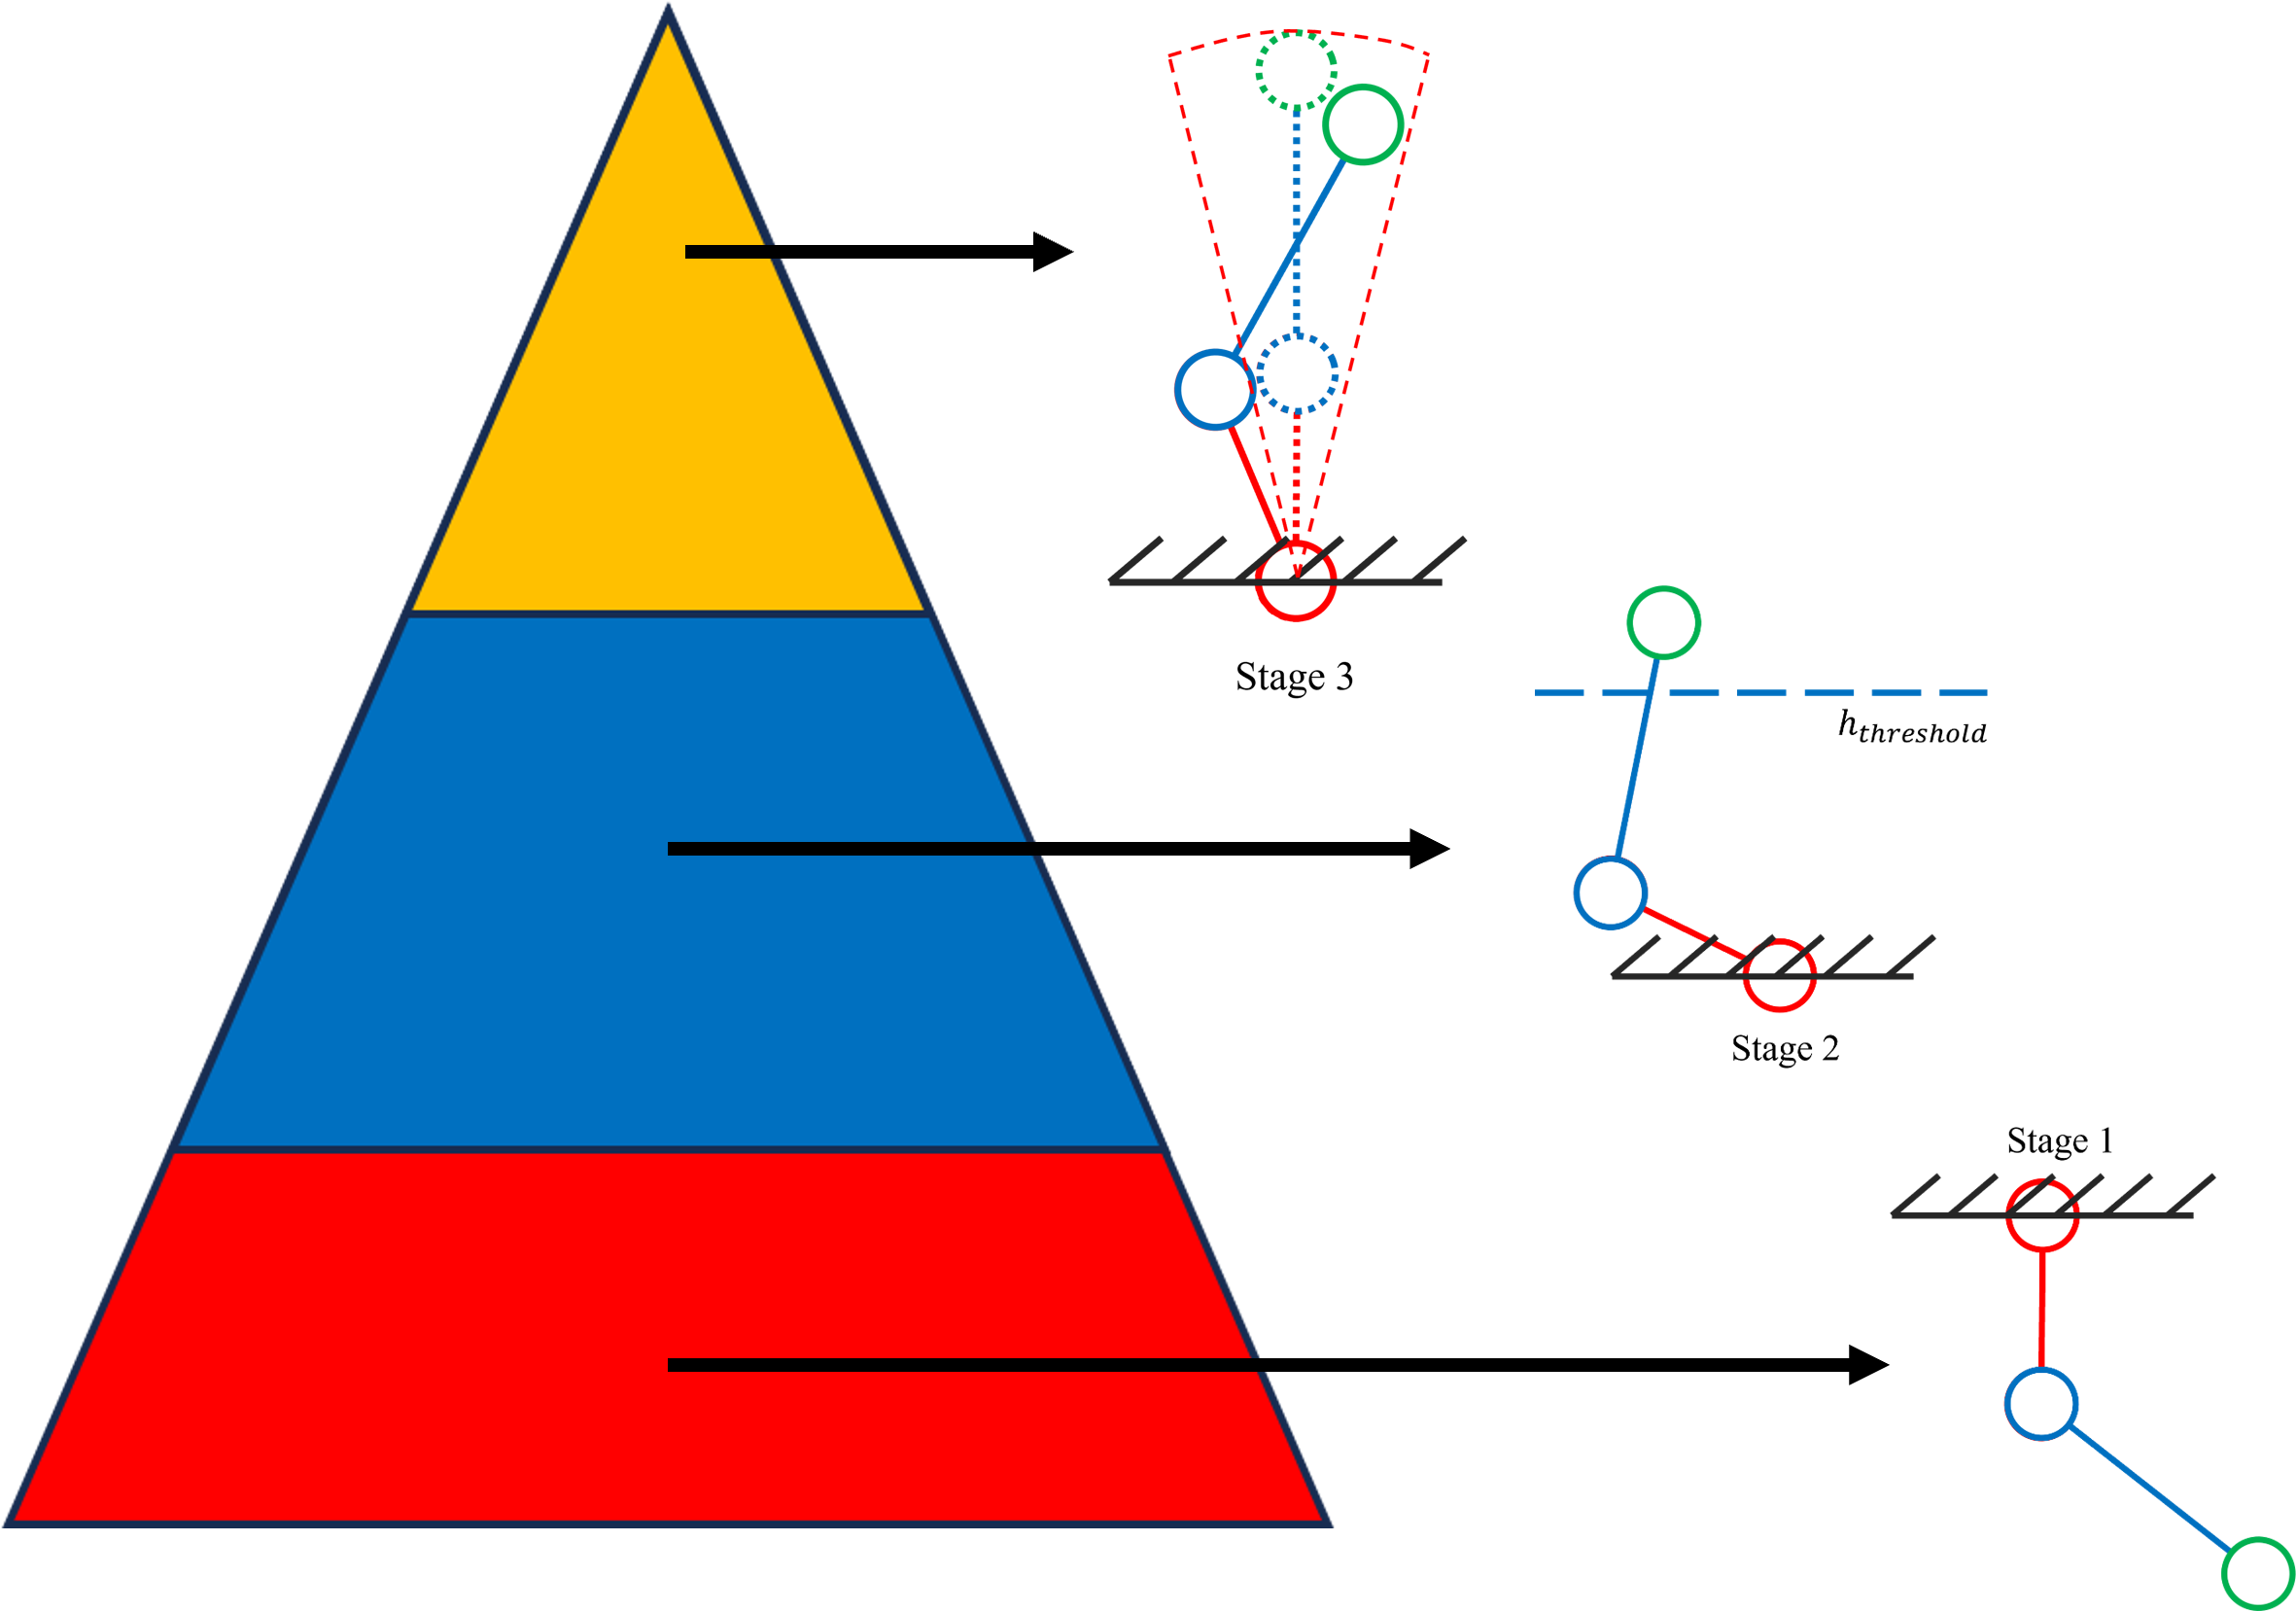
\includegraphics[width=0.9\textwidth]{figures/reward_explained.png} % Adjust the width as needed
    \caption{Interpretation of reward shaping}
    \label{fig:example}
\end{figure}

\cleardoublepage
